\documentclass[conference,compsoc]{IEEEtran}
\usepackage{amsmath,amsfonts,amssymb}
\usepackage{algorithmic}
\usepackage{algorithm}
\usepackage{array}
\usepackage[caption=false,font=footnotesize,labelfont=sf,textfont=sf]{subfig}
\usepackage{textcomp}
\usepackage{stfloats}
\usepackage{url}
\usepackage{verbatim}
\usepackage{graphicx}
\usepackage[nocompress]{cite}
\usepackage{listings}
\usepackage{xcolor}
\usepackage[catalan]{babel}
\usepackage[T1]{fontenc}
\usepackage[utf8]{inputenc}
\usepackage{booktabs}
\usepackage{float}
\usepackage{cuted}
\usepackage{wrapfig}
\usepackage{multirow}
\usepackage{microtype}
\usepackage{siunitx}
\usepackage{pgfplots}
\pgfplotsset{compat=1.18}
\graphicspath{{./}{P3/memoria/}}

% Catalan names for abstract and index terms
\renewcommand{\abstractname}{Resum}
\renewcommand{\IEEEkeywordsname}{Termes d'índex}

% Abstract and IEEEkeywords: bold label, normal-weight body text
\makeatletter
\def\abstract{\normalfont\@IEEEtweakunitybaselinestretch{1.15}%
    \if@twocolumn
      \@IEEEabskeysecsize\noindent\textbf{\textit{\abstractname}}---\normalfont\@IEEEabskeysecsize\relax
    \else
      \bgroup\par\addvspace{0.5\baselineskip}\centering\vspace{-1.78ex}\@IEEEabskeysecsize\textbf{\abstractname}\par\addvspace{0.5\baselineskip}\egroup\quotation\normalfont\@IEEEabskeysecsize%
    \fi\@IEEEgobbleleadPARNLSP}
\def\IEEEkeywords{\normalfont\@IEEEtweakunitybaselinestretch{1.15}%
    \if@twocolumn
      \@IEEEabskeysecsize\vskip 0.5\baselineskip plus 0.25\baselineskip minus 0.25\baselineskip\noindent
      \textbf{\textit{\IEEEkeywordsname}}---\normalfont\@IEEEabskeysecsize\relax
    \else
      \bgroup\par\addvspace{0.5\baselineskip}\centering\@IEEEabskeysecsize\textbf{\IEEEkeywordsname}\par\addvspace{0.5\baselineskip}\egroup\quotation\normalfont\@IEEEabskeysecsize%
    \fi\@IEEEgobbleleadPARNLSP}
\makeatother

% Configuració de listings per a Java
\lstset{
    language=Java,
    basicstyle=\ttfamily\footnotesize,
    keywordstyle=\color{blue}\bfseries,
    commentstyle=\color{gray}\itshape,
    stringstyle=\color{red!70!black},
    numbers=left,
    numberstyle=\tiny\color{gray},
    numbersep=5pt,
    frame=single,
    breaklines=true,
    showstringspaces=false,
    tabsize=4,
    captionpos=b
}

\hyphenation{al-go-ris-me al-go-ris-mes di-vi-deix con-que-rir dis-tri-bu-ció buc-ket}

\begin{document}

\title{Parella de Punts Més Propera i Més Llunyana\\ Pràctica 3}

\author{\IEEEauthorblockN{Serafí Nebot Ginard}
\IEEEauthorblockA{Universitat de les Illes Balears (UIB)\\
Grau en Enginyeria Informàtica\\
Algorismes Avançats, Curs 2025--2026}}

\maketitle

\begin{strip}
\begin{abstract}
Aquesta memòria descriu el disseny i la implementació d'una aplicació Java
que resol el problema de la parella de punts més propera (\textit{closest pair})
i més llunyana (\textit{farthest pair}) sobre un conjunt de punts en el pla.
S'implementen quatre algorismes: força bruta $O(n^2)$, divideix i
venceràs amb franja ordenada $O(n \log^2 n)$, una variant amb \textit{buckets},
i la parella més llunyana mitjançant \textit{convex hull} i
\textit{rotating calipers} $O(n \log n)$.
L'aplicació separa la lògica, la interfície gràfica i el control en tres capes independents, ofereix una interfície gràfica interactiva
amb visualització dels punts i resultats, i incorpora una eina de benchmark
amb gràfiques i predicció de temps.
Es presenta una anàlisi experimental rigorosa que confirma les complexitats
teòriques i revela que l'optimització per \textit{buckets} no aporta guany
pràctic per al problema de la parella més propera.
\end{abstract}

\begin{IEEEkeywords}
parella més propera, parella més llunyana, divideix i venceràs, força bruta,
convex hull, rotating calipers, Model-Vista-Controlador, benchmark, Java Swing
\end{IEEEkeywords}
\end{strip}

\IEEEpeerreviewmaketitle

%% ================================================================
\section{Introducció}

El problema de la parella de punts més propera (\textit{closest pair problem})
és un problema fonamental de la geometria computacional: donat un conjunt
de $n$ punts en el pla, trobar la parella de punts amb la distància
euclidiana mínima. La solució per força bruta examina totes les
$\binom{n}{2}$ parelles amb cost $O(n^2)$, però l'algorisme de divideix
i venceràs redueix el cost a quasi lineal; en aquesta implementació
la franja s'ordena a cada nivell, donant $O(n \log^2 n)$ \cite{ref_gfg_closest}.

El problema complementari, la parella més llunyana (\textit{farthest pair}),
té la mateixa complexitat òptima $O(n \log n)$ però utilitza una
estratègia diferent: primer es construeix el polígon convex que envolta
tots els punts del núvol (\textit{convex hull}) i després s'aplica la tècnica dels
\textit{rotating calipers} \cite{ref_gfg_convex}.

L'aplicació implementada permet generar núvols de punts amb quatre
distribucions (uniforme, gaussiana, exponencial, agrupada), modificar paràmetres d'aquestes,
executar els quatre algorismes, visualitzar els resultats gràficament i
realitzar benchmarks sistemàtics amb predicció de temps.

%% ================================================================
\section{Descripció de l'Aplicació}

L'aplicació és una eina interactiva d'escriptori (Java Swing) que
permet generar núvols de punts, trobar la parella més propera i més
llunyana, i comparar el rendiment dels algorismes. La interfície es
divideix en tres zones: un panell de controls a la part superior,
la visualització de punts al centre i un panell de resultats a la dreta.

\subsection{Generació de Punts}

L'usuari configura el nombre de punts $n$
amb un \textit{spinner} i selecciona una de les quatre distribucions
disponibles. Cada distribució té paràmetres configurables que es
mostren dinàmicament:

\begin{itemize}
    \item \textbf{Uniforme:} punts distribuïts uniformement dins del
          rang $[\texttt{min}, \texttt{max}]$ en ambdós eixos.
    \item \textbf{Gaussiana:} paràmetres de mitjana (fracció del rang),
          desviació estàndard $\sigma$ (fracció del rang) i multiplicadors
          independents per a cada eix, permetent distribucions
          el·líptiques.
    \item \textbf{Exponencial:} factors $\lambda_x$ i $\lambda_y$ que
          controlen la densitat de punts cap a l'origen.
    \item \textbf{Agrupada (\textit{Clustered}):} nombre de clusters
          (mínim 3), amb centres generats uniformement i punts
          distribuïts amb una gaussiana al voltant de cada centre.
\end{itemize}


\subsection{Visualització del Núvol de Punts}

El panell central mostra el núvol de punts generat. Cada punt es
representa com un cercle sòlid de 4~px en gris fosc. El domini de
coordenades $[0, 1000]^2$ es transforma linealment a les coordenades
de pantalla amb un marge de 30~px a cada costat.

Quan s'executen els algorismes, les parelles resultants es ressalten
sobre el núvol: la parella més propera en vermell i la més llunyana
en blau. Cada ressaltat consisteix en una línia que connecta els dos
punts i cercles de 8~px als extrems per destacar-los del núvol.


\subsection{Execució i Resultats}

El botó \textit{Executar} llança els quatre algorismes en un fil
de fons per no bloquejar la interfície. Durant l'execució, els controls
es deshabiliten i el cursor canvia a mode d'espera. El botó
\textit{Aturar} permet cancel·lar l'execució cooperativament.

El panell de resultats a la dreta de la finestra mostra, per a cada
algorisme, les coordenades i distància de la parella trobada i el
temps d'execució mesurat. Mentre no s'ha executat cap algorisme, tots
els valors mostren «---».

Cada algorisme s'executa amb el protocol de la Secció~\ref{sec:benchmark}:
escalfament JIT global al principi de la sèrie i, després, 1 execució
mesurada per cas (algorisme, $n$).


\subsection{Finestra de Benchmark}

El botó \textit{Benchmark} obre una finestra independent no modal per
executar benchmarks sistemàtics. La finestra s'organitza en quatre zones:

\begin{itemize}
    \item \textbf{Configuració (superior):} camps per introduir els valors
          de $n$ separats per comes, un selector de distribució i els
          paràmetres de la distribució triada.
    \item \textbf{Gràfica (centre):} mostra les quatre corbes de temps en
          funció de $n$. Permet activar escala logarítmica i amagar
          series individuals. Superposa corbes ajustades (línia discontínua)
          un cop finalitzat el benchmark.
    \item \textbf{Predicció (dreta):} un cop finalitzat el benchmark,
          ajusta les constants multiplicatives dels models teòrics i
          permet introduir un valor de $n$ arbitrari per predir el
          temps d'execució de cada algorisme.
    \item \textbf{Taula de dades (inferior):} mostra els temps mesurats
          per a cada $n$ i algorisme en format tabular.
\end{itemize}


%% ================================================================
\section{Disseny i Implementació}

\subsection{Estructura de l'Aplicació}

L'aplicació es divideix en tres capes amb responsabilitats ben separades,
que es comuniquen per events:

\begin{enumerate}
    \item \textbf{Model}: la classe \texttt{Model} encapsula el núvol de punts,
          els resultats de cada algorisme (parella i temps), i els
          resultats del benchmark. Només emmagatzema dades; els
          algorismes viuen en classes separades dins la mateixa capa.
    \item \textbf{Vista}: conjunt de components Swing que presenten
          els controls, la visualització i la gràfica. No contenen
          lògica de negoci ni dades del problema.
    \item \textbf{Controlador}: implementa la
          interfície \texttt{ViewListener} per rebre els events de
          la vista, gestiona el cicle de vida dels fils de fons i
          actualitza el model i la vista.
\end{enumerate}

La interfície \texttt{ViewListener} defineix quatre events:
\texttt{onGenerate}, \texttt{onRun}, \texttt{onStop} i
\texttt{onOpenBenchmark}. La vista emet events sense conèixer qui
els processa, i el controlador implementa la interfície sense
conèixer els components gràfics interns de la vista.

Degut a que la vista actualitza automàticament el núvol de punts
cada vegada que l'usuari modifica qualque dada de configuració,
existeix un temporitzador \textit{debounce} de 300~ms que evita emetre l'event
\texttt{onGenerate} a cada tecleig: la vista només el llança quan
l'usuari ha deixat d'interactuar durant 300~ms.

\begin{figure}[h]
    \centering
    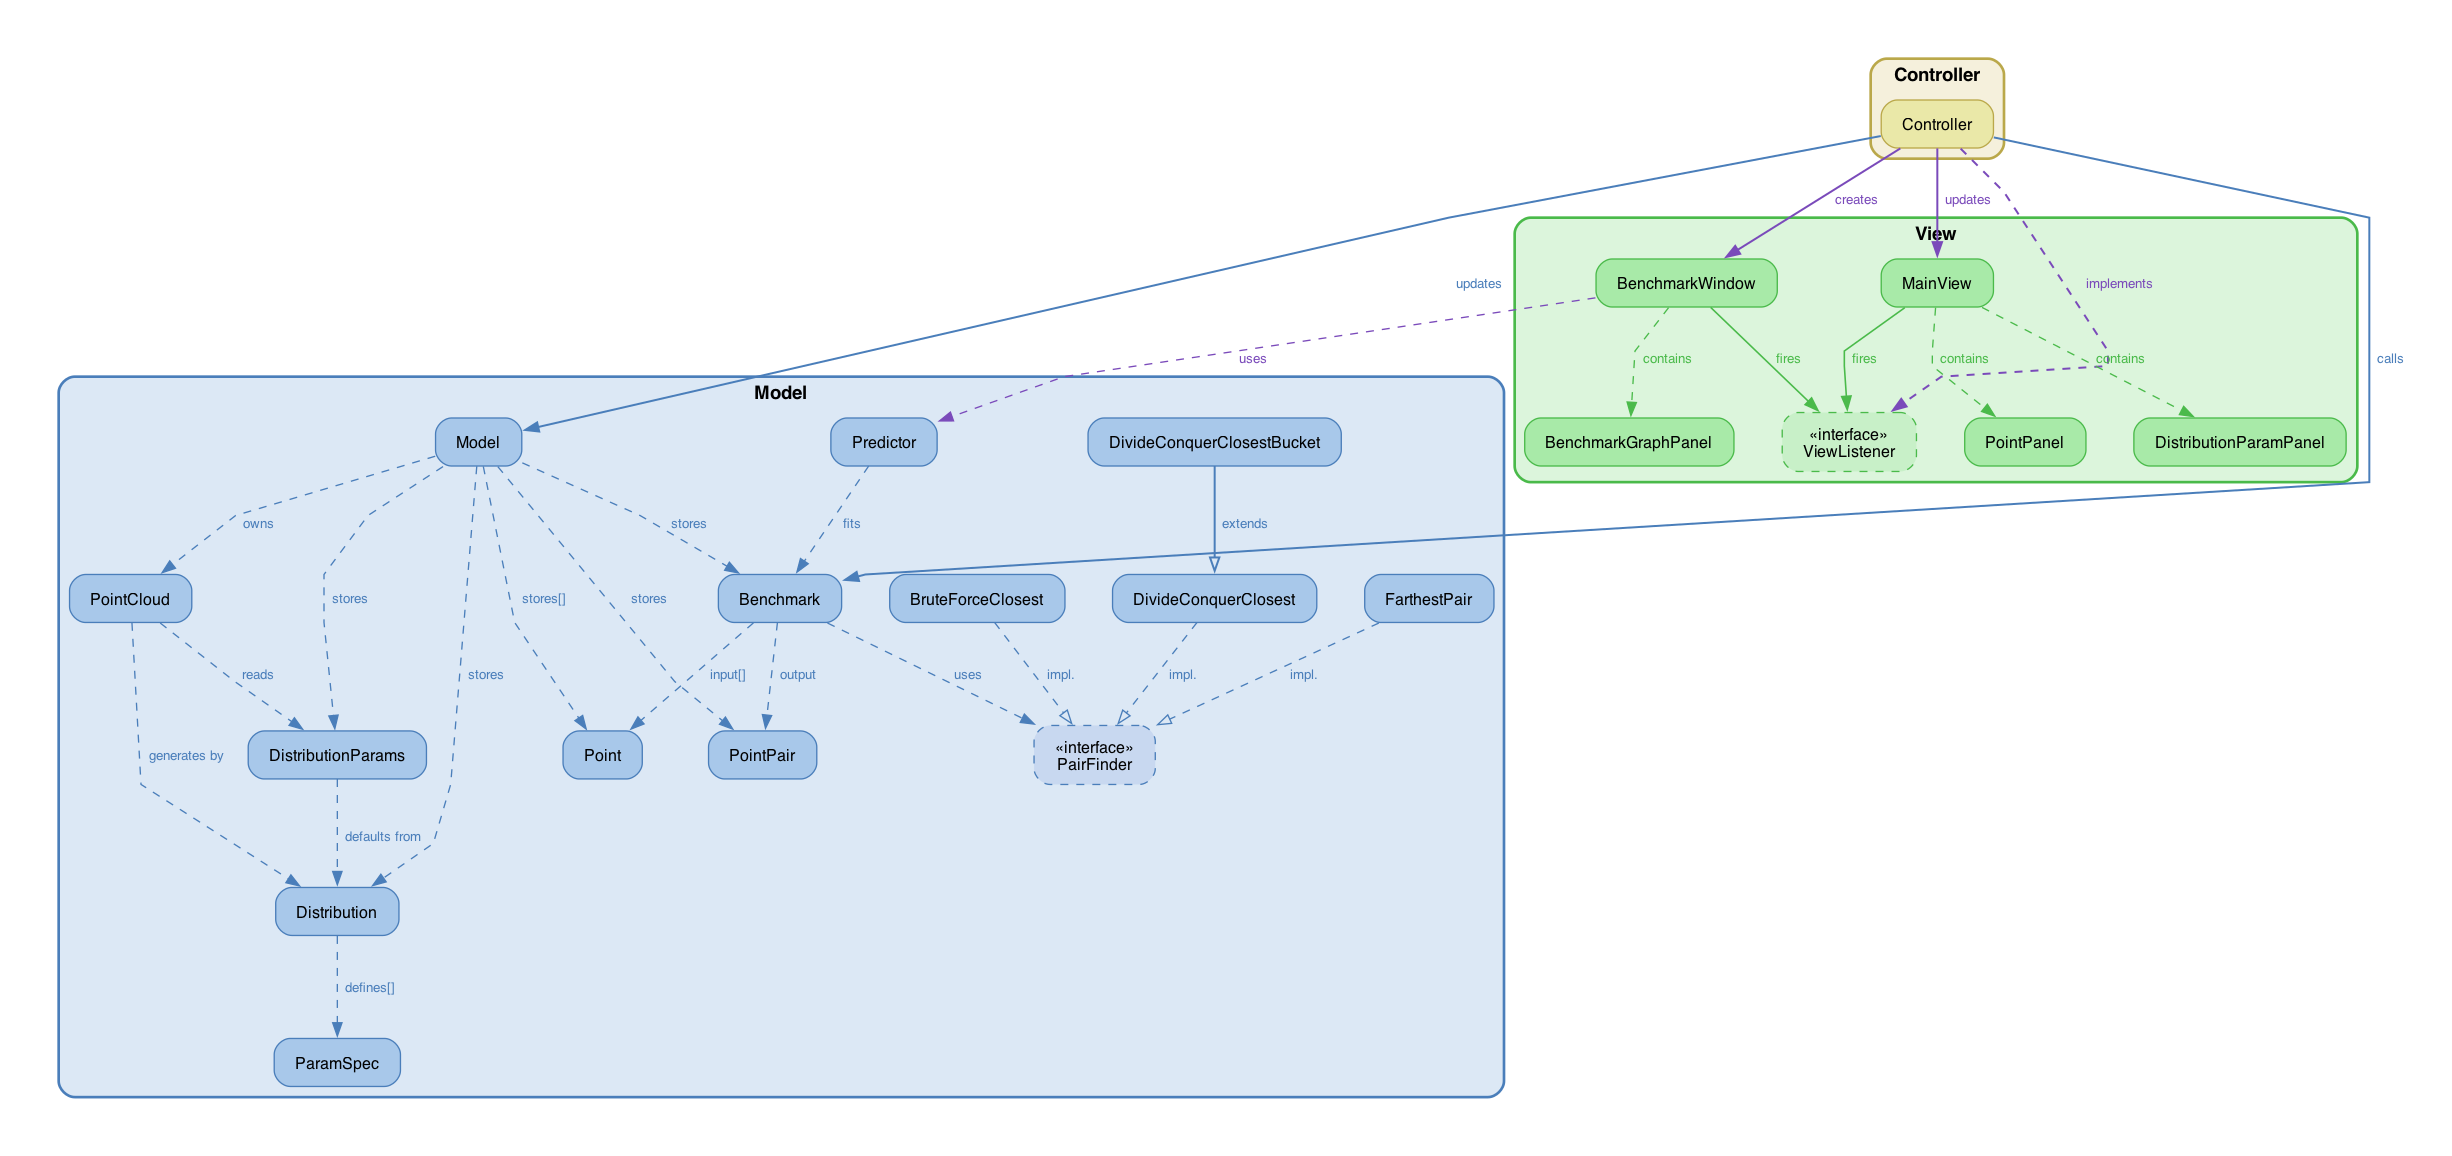
\includegraphics[width=\linewidth]{mvc}
    \caption{Diagrama de classes de l'aplicació amb les relacions entre les tres capes.}
    \label{fig:mvc}
\end{figure}

\subsection{Capa del Model}

La capa del model conté les classes de dades i els algorismes. No
importa cap classe de la vista ni del controlador.

\subsubsection{Model}

La classe \texttt{Model} és el contenidor central d'estat de
l'aplicació. Emmagatzema el núvol de punts actual (\texttt{Point[]}),
la distribució i els paràmetres usats per generar-lo
(\texttt{Distribution}, \texttt{ParamSpec}/\texttt{DistributionParams}),
els resultats de cada algorisme (\texttt{PointPair} i temps en ms)
i els resultats del darrer benchmark (\texttt{BenchmarkEntry[]}).
No conté cap lògica d'algorisme: és un magatzem de dades pur que el
controlador escriu i la vista llegeix a través dels mètodes
d'accés.

\subsubsection{Point i PointPair}

\texttt{Point} és un registre immutable amb dos camps \texttt{double}
(x, y). Ofereix \texttt{distanceTo()} que calcula la distància
euclidiana entre dos punts.

\texttt{PointPair} encapsula una parella de punts i calcula la
distància de forma \textit{lazy}: el camp
\texttt{distance} s'inicialitza a $-1$ com a sentinella i es calcula
només la primera vegada que es demana. Gràcies a això, els algorismes
que construeixen molts \texttt{PointPair} intermedis només paguen el
cost de l'arrel quadrada quan realment es necessita la distància.

\subsubsection{Distribution, PointCloud, DistributionParams i ParamSpec}

L'enumeració \texttt{Distribution} defineix les distribucions disponibles
(uniforme, gaussiana, exponencial i agrupada) i el seu nom de presentació.
\texttt{PointCloud} implementa aquestes distribucions usant
\texttt{java.util.Random}.

Els paràmetres de cada distribució es defineixen com a arrays de
\texttt{ParamSpec} (registre amb nom i valor per defecte), i els
valors actuals s'encapsulen en \texttt{DistributionParams} (registre
immutable amb còpia defensiva al constructor). Aquest disseny permet
que la vista construeixi els camps de configuració automàticament
a partir de \texttt{ParamSpec[]}, sense conèixer quines distribucions
existeixen ni quants paràmetres té cadascuna. D'aquesta forma, si en el
futur s'afageix, elimina o es modifica qualque distribució o paràmetre
no fa falta modificar la vista, aquesta mostrarà totes les opcions automàticament.

\subsubsection{Benchmark i Predictor}
\label{sec:benchmark}

La classe \texttt{Benchmark} centralitza el protocol de mesura i
l'execució paral·lela. El protocol és:

\begin{enumerate}
    \item \textbf{Escalfament JIT global:} s'executen tots els algorismes
          10 vegades amb $n = 500$ abans d'iniciar una sèrie de benchmark
          (finestra/CLI) per forçar la compilació JIT i així descartar possibles
          interferències amb el temps d'execució mesurat.
    \item \textbf{Mesura:} una execució mesurada amb
          \texttt{System.nanoTime()}, convertida a mil·lisegons.
\end{enumerate}
Per a l'execució individual des de la interfície principal s'aplica
directament la fase de mesura.

Per al benchmark en sèrie, \texttt{Benchmark.runSeries} genera els
arrays de punts una sola vegada al fil principal i després distribueix
les tasques amb un \texttt{ExecutorService} de granularitat fina:
una tasca per parella (algorisme, $n$), de manera que els quatre
algorismes per al $n$ més gran s'executen en paral·lel en nuclis
separats.

La classe \texttt{Predictor} ajusta una constant multiplicativa $a$
per a cada algorisme amb mínims quadrats ponderats (sense ordenada a
l'origen):
\begin{equation}
a = \frac{\sum_i t_i \cdot f(n_i)}{\sum_i f(n_i)^2}
\end{equation}
on $n_i$ i $t_i$ són la quantitat de punts del núvol i el temps d'execució mesurat
per a l'execució $i$ del benchmark. La funció $f(n_i)$ equival al temps teòric
per a cada un dels algorismes. La ponderació dóna més pes
a les mesures amb $n$ gran, on el comportament asimptòtic domina la sobrecàrrega
de la JVM.

\subsubsection{Interfície Comuna dels Algorismes}

Tots els algorismes implementen la mateixa interfície \texttt{PairFinder}:

\begin{lstlisting}[caption={Interfície comuna per a tots els algorismes.},label={lst:pairfinder}]
public interface PairFinder {
    PointPair find(Point[] points);
}
\end{lstlisting}

Això permet al benchmark i al controlador cridar qualsevol algorisme
sense saber quin és concretament.

Pel que fa a les dues variants de D\&C, \texttt{DivideConquerClosest}
implementa l'algorisme complet (ordenar per X, recursió, construir franja,
processar franja). \texttt{DivideConquerClosestBucket} en reutilitza
tot menys l'últim pas: sobreescriu només el mètode \texttt{processStrip()}
per usar \textit{buckets} en lloc d'ordenar per Y. D'aquesta manera
no es repeteix cap codi: tot el que és comú entre les dues variants
viu en un sol lloc.

\subsubsection{Algorisme de Força Bruta}

L'algorisme de força bruta (\texttt{BruteForceClosest}) examina totes
les $\binom{n}{2} = \frac{n(n-1)}{2}$ parelles de punts i retorna
la de distància mínima.

\begin{lstlisting}[caption={Nucli de l'algorisme de força bruta.},label={lst:brute}]
for (int i = 0; i < n - 1; i++) {
    for (int j = i + 1; j < n; j++) {
        double dist = points[i].distanceTo(points[j]);
        if (dist < bestDist) {
            bestDist = dist;
            bestP1 = points[i];
            bestP2 = points[j];
        }
    }
}
\end{lstlisting}

\textbf{Cost temporal.} L'algorisme avalua totes les
$\binom{n}{2}=\frac{n(n-1)}{2}$ parelles, per tant
$T(n)\in O(n^2)$.

\textbf{Cost espacial.} L'espai addicional és constant, ja que només
es mantenen variables auxiliars i la millor parella:
$O(1)$.

\textbf{Notes pràctiques.} La implementació comprova
\texttt{Thread.interrupted()} a cada iteració del bucle extern per
permetre la cancel·lació cooperativa des de la interfície. La mateixa
estratègia (amb punts de comprovació adaptats a cada bucle/recursió)
s'aplica també a D\&C, D\&C Bucket i parella llunyana.

\subsubsection{Algorisme de Divideix i Venceràs}
\label{sec:dc}

L'algorisme de divideix i venceràs (\texttt{DivideConquerClosest})
segueix les següents passes:

\begin{enumerate}
    \item Ordenar els punts per coordenada $x$ una sola vegada ($O(n \log n)$).
    \item Recursivament trobar la parella més propera a la meitat
          esquerra i la meitat dreta.
    \item Construir la franja central de punts amb $|x - x_{\text{mid}}| < d_{\min}$.
    \item Processar la franja: ordenar per $y$ i per a cada punt,
          comparar amb els 7 veïns següents (argument de l'empaquetament).
\end{enumerate}

El cas base s'activa quan el subproblema té 3 o menys punts, resolent-se
per força bruta amb cost $O(1)$.

\textbf{Argument d'empaquetament (per què 7 veïns).}
Després de resoldre les dues meitats, $d_{\min}$ és la millor distància
dins de cada costat. En la franja central (amplada $2d_{\min}$), per a un
punt fixat només poden ser candidats els punts amb diferència en $y$ menor
que $d_{\min}$. Això defineix un rectangle de mida
$2d_{\min} \times d_{\min}$. Si el subdividim en cel·les de costat
$d_{\min}/2$, obtenim 8 cel·les; no hi pot haver dos punts a la mateixa
cel·la perquè estarien a distància menor que $d_{\min}$ (contradicció).
Per tant, hi ha com a màxim 8 punts rellevants en aquesta zona i,
ordenant per $y$, n'hi ha prou de comparar cada punt amb els 7 següents.
Aquest límit constant (6--8 segons la formulació geomètrica) és la clau
del cost lineal de la franja \cite{ref_gfg_closest}.

\textbf{Cost temporal.}
Podem expressar el cost de la funció recursiva de la següent forma:
\begin{equation}
T(n)=2T(n/2)+f(n)
\end{equation}
on $f(n) \in O(n\log n)$ prové del processament de la franja a cada nivell:
ordenació per $y$ ($O(k\log k)$ amb $k \leq n$) i comparacions acotades entre veïns
a la franja (cost lineal sobre $k$, amb un màxim constant de comparacions
per punt).

Podem resoldre la recurrència amb el \textit{Teorema Mestre}:
\[
T(n)=a\,T\!\left(\frac{n}{b}\right)+f(n)
\]
on $a$ és el nombre de subproblemes, $n/b$ la mida de cada subproblema,
i $f(n)$ el cost de combinar resultats.

En el nostre cas:
\begin{itemize}
    \item $a=2$ (dues meitats),
    \item $b=2$ (cada meitat té mida $n/2$),
    \item $f(n)=n\log n$ (cost de processar la franja).
\end{itemize}

Com que el treball recursiu pur és d'ordre $n$ (ja que
$n^{\log_b a}=n^{\log_2 2}=n$) i aquí la combinació és un factor
$\log n$ més gran ($n\log n$), la forma generalitzada del Teorema
Mestre dona:
\[
T(n)\in O(n\log^2 n)
\]

\textbf{Cost espacial.} L'espai és
$O(n)$ (buffer de franja preallocat + pila recursiva).

\textbf{Notes pràctiques.} Les optimitzacions següents no canvien
l'ordre asimptòtic, però redueixen constants i milloren el rendiment
real de l'algorisme.

\textbf{Optimització 1 -- Cerca binària per als límits de la franja.}

En lloc d'un escaneig lineal $O(k)$ per trobar els punts dins de la
franja, s'utilitza cerca binària $O(\log k)$ amb els mètodes
\texttt{lowerBound} i \texttt{upperBound}, aprofitant que els punts
ja estan ordenats per $x$. Això no millora la complexitat
asimptòtica (el pas dominant segueix sent l'ordenació de la franja)
però redueix el treball constant.

\textbf{Optimització 2 -- Buffer preallocat per a la franja.}

A cada nivell de recursió, l'algorisme necessita copiar els punts
de la franja central a un buffer temporal per ordenar-los per $y$.
La implementació ingènua crearia un nou array a cada crida recursiva,
generant $O(\log n)$ al·locacions (una per nivell).

Per eliminar la pressió sobre el \textit{garbage collector} i millorar
la localitat de cache, s'al·loca un únic array \texttt{Point[n]} al
mètode \texttt{find()} i es reutilitza a tots els nivells de recursió.
El buffer és segur perquè cada nivell de recursió l'omple amb
\texttt{System.arraycopy} i només accedeix als índexos $[0, k)$
on $k$ és el nombre de punts de la franja actual. Els nivells de
recursió no es trepitgen perquè l'execució és seqüencial (un sol fil):
un nivell pare copia la seva franja, fa la crida al nivell fill i queda
aturat fins que el fill retorna. Si el fill sobreescriu el buffer, no
passa res: el pare ja no necessita les dades antigues.

\subsubsection{Variant amb Buckets}
\label{sec:bucket}

La variant amb \textit{buckets} (\texttt{DivideConquerClosestBucket})
intenta millorar el pas de processament de la franja. En lloc
d'ordenar la franja per $y$ amb cost $O(k \log k)$, distribueix els
punts en cubetes (\textit{buckets}) d'alçada $d_{\min}$ i comprova
només la cubeta actual i la immediatament superior. Per l'argument de
l'empaquetament explicat abans, cada cubeta conté com a màxim 8 punts, de manera
que el cost per punt és $O(1)$ i el cost total de la franja és $O(k)$.

\textbf{Cost temporal.} La millora damunt del D\&C fa que la recurrència es redueixi de
$T(n) = 2T(n/2) + k \log k$ a $T(n) = 2T(n/2) + k$.
Com que $k \leq n$, llavors $T(n)\in O(n \log n)$.

\textbf{Cost espacial.} El consum addicional és lineal en el pitjor cas
($O(n)$ per al buffer i estructures de franja), però amb constants més
altes que D\&C per la gestió de cubetes.

\textbf{Notes pràctiques.}Cost de Cubetes Disperses.
L'optimització per \textit{buckets} requereix crear un array de
cubetes indexat pel rang de coordenada $y$. El nombre de cubetes
és:
\begin{equation}
\texttt{numBuckets} = \left\lfloor \frac{y_{\max}}{d_{\min}} \right\rfloor - \left\lfloor \frac{y_{\min}}{d_{\min}} \right\rfloor + 1
\end{equation}

Quan $\texttt{numBuckets} \gg k$ (molt més cubetes que punts), la
representació en memòria esdevé molt dispersa: es creen vectors de
grandària proporcional a \texttt{numBuckets} (p.~ex.\
\texttt{buckets[numBuckets * 8]} i \texttt{counts[numBuckets]}), però
només s'omplen $k$ posicions útils. Això implica dos efectes pràctics:
(1) sobrecost d'al·locació/inicialització d'estructures grans i
(2) pitjor localitat espacial, perquè es recorren moltes cubetes buides
entre poques cubetes amb dades. En conseqüència augmenten les fallades
de cache i la pressió de memòria, i el guany teòric del pas lineal queda
neutralitzat o superat. Aquest patró també apareix en índexs espacials
basats en graella i \textit{spatial hashing}.

Per a evitar aquest problema, es podria afegir una guarda
(p.~ex.\ \texttt{if (numBuckets > k)}) per fer \textit{fallback} al
processament clàssic de franja. Aquesta decisió reduiria el sobrecost
de memòria, però també faria que la variant bucket es comporti com el
D\&C normal en la majoria de casos pràctics. A n'aquesta implementació no s'ha
introduït cap guarda per a mantenir el comportament de la variant de \textit{buckets}.

\subsubsection{Parella Més Llunyana}

L'algorisme de la parella més llunyana (\texttt{FarthestPair})
combina dues tècniques: \textit{convex hull} i
\textit{rotating calipers} \cite{ref_gfg_convex}.

\textbf{Fase 1 -- \textit{Convex hull} (envolupant convexa).}
Primer s'ordenen els punts per coordenada $x$ i es construeix la
frontera exterior del núvol: polígon convex que conté la resta de punts al seu interior.
El codi ho fa en dues
passades (cadena inferior i cadena superior), eliminant els punts que
fan gir no convex. El resultat és una llista ordenada de vèrtexs de la
frontera; tots els punts interiors queden descartats perquè no poden ser
extrems de la distància màxima. L'ordenació inicial domina el cost
amb $O(n\log n)$; la construcció de les dues cadenes és lineal. Per tant,
el cost de la fase és $O(n\log n)$.

\textbf{Fase 2 -- \textit{Rotating calipers}.}
Sobre la frontera convexa, es mantenen dos índexs (dos ``calipers'') i
es recorren els vèrtexs buscant parelles antipodals. A cada pas es
compara l'àrea orientada del costat actual amb el següent per decidir
quin punter avançar. Això evita provar totes les parelles de vèrtexs:
cada punter fa una volta com a màxim, de manera que la cerca sobre
l'envolupant és lineal. Si $h$ és el nombre de vèrtexs de
l'envolupant convexa, cada punter avança com a màxim $h$ posicions i el
cost és $O(h)$ (amb $h\leq n$).

En resum funcional, el procés és:
\begin{enumerate}
    \item Reduir el problema als vèrtexs de la frontera (\textit{convex hull}).
    \item Cercar la millor parella només entre aquests vèrtexs
          (\textit{rotating calipers}).
\end{enumerate}

\textbf{Cost temporal.} Com que el \textit{convex hull} costa
$O(n \log n)$ i els \textit{rotating calipers} costen $O(h)$,
el cost total és $T(n)\in O(n \log n)$.

\textbf{Cost espacial.} L'espai addicional és lineal per
emmagatzemar l'envolupant convexa i estructures auxiliars:
$O(n)$. La raó és que, en el pitjor cas, tots els punts poden formar
part de l'envolupant (per exemple, si ja estan sobre una frontera
convexa), de manera que cal guardar fins a $n$ vèrtexs. A més, les
estructures temporals de construcció (cadenes inferior/superior) també
contenen com a màxim una quantitat proporcional a $n$ punts.

\subsection{Capa de la Vista}

La capa de la vista consta de cinc components Swing principals, cadascun
amb una responsabilitat concreta.

\subsubsection{MainView}

La finestra principal usa \texttt{BorderLayout}: el panell de controls a
dalt (\texttt{NORTH}), el \texttt{PointPanel} al centre i el panell de
resultats a la dreta (\texttt{EAST}). El panell de controls combina
dos subpanells amb \texttt{FlowLayout}: un a l'esquerra amb el
\texttt{JSpinner} de $n$, el \texttt{JComboBox} de distribució i el
\texttt{DistributionParamPanel}, i un a la dreta amb els botons
\textit{Executar}, \textit{Aturar} i \textit{Benchmark}.

La comunicació cap al controlador es fa exclusivament a través de
\texttt{ViewListener}: el botó \textit{Executar} crida \texttt{onRun},
\textit{Aturar} crida \texttt{onStop}, i \textit{Benchmark} crida
\texttt{onOpenBenchmark}. La vista no coneix el controlador; simplement
invoca l'event sobre el listener registrat.

El panell de resultats organitza vuit etiquetes en vertical amb
\texttt{BoxLayout}: quatre per a les parelles trobades (coordenades i
distància) i quatre per als temps d'execució. Quan s'ha generat un
núvol nou però encara no s'han executat algorismes, les etiquetes
mostren «---» i el botó \textit{Executar} s'habilita per indicar que
les dades estan llestes.

\subsubsection{PointPanel}

El panell on es mostra el núvol de punts generat i la solució trobada
per a la distància mínima i màxima.
El renderitzat es fa directament a \texttt{paintComponent} amb tres
capes seqüencials: primer tots els punts del núvol en gris, després la
parella llunyana en blau (si disponible) i finalment la parella propera
en vermell (si disponible).

La transformació de domini a pantalla és:
\begin{align}
x_{\text{px}} &= \texttt{MARGIN} + \frac{x - x_{\min}}{x_{\max} - x_{\min}} \cdot w \\
y_{\text{px}} &= \texttt{MARGIN} + h - \frac{y - y_{\min}}{y_{\max} - y_{\min}} \cdot h
\end{align}
on $w$ i $h$ són les dimensions útils del panell (descomptant els marges).
Els valors $x_{\min}, x_{\max}, y_{\min}, y_{\max}$ representen els límits
del domini de dades (mínim i màxim de cada eix) utilitzats per normalitzar
les coordenades abans de pintar-les.
La resta de $h$ a la fórmula de $y$ inverteix l'eix perquè la
pantalla té l'origen a dalt i el domini matemàtic a baix.

\subsubsection{DistributionParamPanel}

Panell auxiliar encarregat de mostrar i editar els paràmetres de la
distribució seleccionada.

Aquest panell genera els seus camps de text dinàmicament en el moment
en què es canvia la distribució seleccionada. Recorre l'array
\texttt{ParamSpec[]} de la distribució i crea un parell \texttt{JLabel}
+ \texttt{JTextField} per a cada paràmetre, inicialitzant-lo amb el valor
per defecte de l'especificació. Cada camp té un \texttt{DocumentListener} que, quan el contingut canvia,
reinicia el temporitzador de \textit{debounce} de \texttt{MainView}, el qual
al seu torn emet l'event \texttt{onGenerate} al \texttt{ViewListener}
un cop transcorreguts els 300~ms. Si l'usuari introdueix un valor no
numèric, el mètode \texttt{read()} retorna silenciosament el valor per
defecte sense mostrar cap error.

Gràcies a aquest disseny, afegir una nova distribució o modificar els
seus paràmetres no requereix cap canvi a la vista.

\subsubsection{BenchmarkWindow}

Finestra secundària on es configura i s'executa el benchmark, i on es
visualitzen els resultats agregats.

La finestra de benchmark és un \texttt{JDialog} no modal. Utilitza
\texttt{BorderLayout} amb la configuració a dalt, la gràfica al centre,
un panell d'opcions i predicció a la dreta, i la taula de dades a baix.

De manera idèntica a \texttt{MainView}, \texttt{BenchmarkWindow} es
comunica amb el controlador a través de \texttt{ViewListener}. El mètode
\texttt{onRunBenchmark()} forma part de la mateixa interfície que
\texttt{onRun}, \texttt{onStop}, etc., de manera que el controlador
és l'únic punt d'implementació i la finestra no coneix en cap moment
el seu tipus concret.

L'execució del benchmark es delega a un \texttt{SwingWorker}. Quan el \texttt{SwingWorker}
acaba, el mètode \texttt{done()} s'executa a l'EDT, actualitza la gràfica,
la taula i ajusta les constants del predictor, i habilita el botó de
predicció.

\subsubsection{BenchmarkGraphPanel}

Component de dibuix encarregat de representar les corbes de temps
mesurat i les corbes ajustades pel predictor.

La gràfica es dibuixa completament a \texttt{paintComponent}, sense
cap llibreria externa. El mètode \texttt{generateRoundTicks()} calcula
etiquetes d'eixos arrodonides a potències de $10 \times \{1, 2, 5\}$
per obtenir graelles netes independentment del rang de valors.

En mode logarítmic, l'eix $y$ es transforma amb $\log_{10}$ i les
divisions secundàries es col·loquen als múltiples $\times 2$ i $\times 5$
de cada potència de $10$. En mode lineal, les divisions es calculen amb
\texttt{generateRoundTicks}.

Les corbes ajustades es dibuixen amb una línia discontínua
(\texttt{BasicStroke} amb array de \textit{dash}) en un to lleugerament
més fosc que la sèrie de dades corresponent, mostrant el model
$a \cdot f(n)$ mostrejat a un píxel per columna.

\subsection{Capa del Controlador}

La capa del controlador consisteix en una sola classe,
\texttt{Controller}, que implementa \texttt{ViewListener} i conté tota
la lògica d'orquestració de l'aplicació.

\subsubsection{Gestió dels Events de la Vista}

Cada mètode de \texttt{ViewListener} correspon a una acció de l'usuari:

\begin{itemize}
    \item \textbf{\texttt{onGenerate}}: crida \texttt{model.generatePoints()}
          amb els paràmetres rebuts, i seguidament
          \texttt{view.showPoints()} per actualitzar la visualització i
          \texttt{view.clearResults()} per esborrar els resultats anteriors.
          Finalment habilita el botó \textit{Executar}.

    \item \textbf{\texttt{onRun}}: crea un \texttt{SwingWorker} que
          executa els quatre algorismes sobre el núvol actual al fil de
          fons, desa els resultats al model amb \texttt{model.setResults()},
          i en acabar crida \texttt{view.updateResults()} a l'EDT.
          Durant l'execució, crida \texttt{view.setRunning(true)} per
          deshabilitar els controls i activar el cursor d'espera.

    \item \textbf{\texttt{onStop}}: crida \texttt{worker.cancel(true)},
          que interromp el fil de fons. La cancel·lació és cooperativa:
          tots els algorismes comproven periòdicament
          \texttt{Thread.isInterrupted()} en punts de control
          (bucles principals i entrades recursives) i llancen una
          excepció quan detecten la interrupció.

    \item \textbf{\texttt{onOpenBenchmark}}: crea la \texttt{BenchmarkWindow}
          (si no existeix ja) passant-se a si mateix com a
          \texttt{ViewListener}, i la fa visible.
\end{itemize}

\subsection{CLI de Benchmark}

A més de la interfície gràfica, s'ofereix una eina de línia de
comandes (\texttt{BenchmarkCLI}) que permet executar benchmarks
amb paràmetres configurables i sortida en format taula o CSV:

El flux d'execució del CLI és el següent:
\begin{enumerate}
    \item Llegeix els paràmetres de consola (distribució, valors de $n$,
          algorismes, nombre de repeticions i format de sortida).
    \item Mostra la configuració seleccionada i fa un escalfament JIT
          inicial amb un conjunt petit de punts.
    \item Per a cada repetició, genera els núvols de punts per a tots els
          valors de $n$ i llança en paral·lel les tasques
          \texttt{(algorisme, n)}.
    \item Recull els temps, en calcula la mitjana entre repeticions i
          imprimeix el resultat final en taula o CSV.
\end{enumerate}

Paràmetres principals:
\begin{itemize}
    \item \texttt{-d/--dist}: distribució (
          \texttt{UNIFORM}, \texttt{GAUSSIAN}, \texttt{EXPONENTIAL}, \texttt{CLUSTERED}).
    \item \texttt{-p/--params}: paràmetres numèrics de la distribució
          (en l'ordre definit per cada distribució).
    \item \texttt{-n/--nvals}: llista de mides de problema separades per comes.
    \item \texttt{-a/--algos}: subconjunt d'algorismes
          (\texttt{brute}, \texttt{dc}, \texttt{bucket}, \texttt{farthest}).
    \item \texttt{-r/--runs}: nombre d'execucions independents per fer mitjana.
    \item \texttt{--csv}: sortida en format CSV (si no, taula textual).
\end{itemize}

Per evitar ambigüitats, la Taula~\ref{tab:cli_param_order} resumeix
l'ordre exacte dels valors a \texttt{-p/--params} per a cada distribució.

\begin{table}[H]
    \caption{Ordre de paràmetres per a \texttt{-p/--params}.\label{tab:cli_param_order}}
    \centering
    \scriptsize
    \begin{tabular}{ll}
        \toprule
        Distribució & Ordre de paràmetres a \texttt{-p} \\
        \midrule
        \texttt{UNIFORM} & \texttt{min,max} \\
        \texttt{GAUSSIAN} & \texttt{mean,sigma,mulX,mulY} \\
        \texttt{EXPONENTIAL} & \texttt{lambdaX,lambdaY} \\
        \texttt{CLUSTERED} & \texttt{clusters,spread} \\
        \bottomrule
    \end{tabular}
\end{table}

\begin{lstlisting}[caption={Exemples d'ús del CLI.},label={lst:cli},language=bash]
# Tots els algorismes, distribucio uniforme
java -cp target/classes \
  com.serafinebot.p3.BenchmarkCLI

# D&C vs Bucket, gaussiana, CSV
java -cp target/classes \
  com.serafinebot.p3.BenchmarkCLI \
  -a dc,bucket -d GAUSSIAN --csv

# 3 execucions promitjades
java -cp target/classes \
  com.serafinebot.p3.BenchmarkCLI -r 3
\end{lstlisting}

%% ================================================================
\section{Anàlisi Experimental}
\label{sec:experimental}

Totes les mesures s'han realitzat amb el CLI de benchmark, amb
3 execucions independents mitjanes. S'han provat les distribucions uniforme, gaussiana
($\mu=0.5$, $\sigma=1/6$), exponencial ($\lambda_x=\lambda_y=5$) i
agrupada (5 clusters). L'execució del benchmark distribueix les tasques
entre nuclis; això pot afegir soroll en temps molt petits però no afecta
les tendències globals. Com a cas addicional s'ha provat una gaussiana
estirada ($\sigma=0.05$, multiplicadors $\times4$ i $\times0.25$).
Els valors analitzats cobreixen des de $n=500$ fins a $n=300\,000$,
amb més densitat de mostres a valors petits i intermedis.
Els temps petits (\textless 0.1~ms)
presenten variabilitat elevada; s'analitzen sobretot tendències i valors
per a $n$ grans.
Cal remarcar que la generació de núvols és aleatòria i, en aquesta versió,
no es fixa una llavor (\textit{seed}) global; per tant, dues execucions amb els mateixos paràmetres
produeixen mostres diferents. Per això es realitzen 3 execucions seguides per a cada configuració
de cada algorisme i es fa feina damunt la seva mitja.

\subsection{Distribució Uniforme: Comparació Completa}

La Taula~\ref{tab:uniform} recull els temps mitjans per a la distribució
uniforme i la Figura~\ref{fig:uniform_plot} mostra el creixement en escala
logarítmica.

\begin{table}[H]
    \caption{Temps d'execució (ms) per a distribució uniforme.\label{tab:uniform}}
    \centering
    \footnotesize
    \begin{tabular}{r S[table-format=6.3] S[table-format=4.3] S[table-format=4.3] S[table-format=4.3]}
        \toprule
        {$n$} & {Bruta} & {D\&C} & {D\&C Bkt.} & {Llunyana} \\
        \midrule
        500    & 0.178 & 0.472 & 1.324 & 0.848 \\
        1000   & 0.685 & 0.889 & 1.137 & 2.331 \\
        5000   & 27.263 & 7.542 & 51.043 & 50.777 \\
        10000  & 171.028 & 18.215 & 28.158 & 28.750 \\
        50000  & 9180.847 & 90.739 & 274.017 & 135.219 \\
        100000 & 36675.313 & 345.969 & 493.501 & 394.892 \\
        150000 & 87350.465 & 596.639 & 1008.263 & 491.157 \\
        200000 & 143702.082 & 878.369 & 1692.344 & 868.165 \\
        250000 & 175852.252 & 1260.477 & 2369.061 & 987.417 \\
        300000 & 209233.170 & 1701.369 & 2783.924 & 1046.394 \\
        \bottomrule
    \end{tabular}
\end{table}

\begin{figure}[H]
    \centering
    \pgfplotstableread[col sep=comma]{
n,brute,dc,bucket,farthest
500,0.177889,0.472306,1.324319,0.847569
1000,0.685319,0.888819,1.137444,2.330833
5000,27.263055,7.542277,51.043292,50.776959
10000,171.027805,18.214708,28.157959,28.750347
50000,9180.846833,90.739125,274.016875,135.218764
100000,36675.313222,345.969319,493.500875,394.892486
150000,87350.464944,596.638889,1008.262986,491.156903
200000,143702.081945,878.368680,1692.344375,868.165195
250000,175852.252195,1260.476556,2369.060861,987.417194
300000,209233.170278,1701.368972,2783.924319,1046.394500
    }\uniformdata
    \begin{tikzpicture}
    \begin{semilogyaxis}[
        width=0.98\linewidth,
        height=6cm,
        xlabel={$n$},
        ylabel={Temps (ms)},
        grid=both,
        legend pos=north west,
        legend style={font=\footnotesize, fill=white, fill opacity=0.85, draw opacity=1},
        mark size=1.8pt
    ]
        \addplot table[x=n,y=brute] {\uniformdata};
        \addlegendentry{Bruta}
        \addplot table[x=n,y=dc] {\uniformdata};
        \addlegendentry{D\&C}
        \addplot table[x=n,y=bucket] {\uniformdata};
        \addlegendentry{D\&C Bucket}
        \addplot table[x=n,y=farthest] {\uniformdata};
        \addlegendentry{Llunyana}
    \end{semilogyaxis}
    \end{tikzpicture}
    \caption{Distribució uniforme: temps vs $n$ (escala logarítmica).}
    \label{fig:uniform_plot}
\end{figure}

Els resultats mostren el patró esperat: força bruta domina per a $n$ petits
per la seva baixa constant, però queda ràpidament superada per D\&C i
la parella llunyana. Per $n=300\,000$, D\&C és $\approx 123\times$ més ràpid
que força bruta, mentre que la parella llunyana és la més ràpida dels algorismes
quasi-lineals. La variant amb \textit{buckets} és sistemàticament més lenta
que D\&C en la distribució uniforme (\textasciitilde 64\% a $n=300\,000$).

\subsection{Comparació entre Distribucions}

La Taula~\ref{tab:distributions} resumeix els temps a $n = 300\,000$ per a
totes les distribucions i el cas gaussià estirat. La Figura~\ref{fig:dist_bar}
mostra la comparativa completa dels quatre algorismes.

\begin{table}[H]
    \caption{Temps (ms) per algorisme i distribució a $n = 300\,000$.\label{tab:distributions}}
    \centering
    \scriptsize
    \begin{tabular}{l S[table-format=6.1] S[table-format=4.1] S[table-format=4.1] S[table-format=4.1]}
        \toprule
        {Distribució} & {Bruta} & {D\&C} & {D\&C Bkt.} & {Llunyana} \\
        \midrule
        Uniforme            & 209233.2 & 1701.4 & 2783.9 & 1046.4 \\
        Gaussiana           & 215653.4 & 1662.1 & 3101.5 & 1195.7 \\
        Exponencial         & 210040.3 & 2021.5 & 4125.5 & 1338.5 \\
        Agrupada (5)        & 209850.6 & 1721.2 & 3322.0 & 1102.0 \\
        Gaussiana est.      & 212501.2 & 1372.6 & 1702.7 & 925.6 \\
        \bottomrule
    \end{tabular}
\end{table}

\begin{figure}[H]
    \centering
    \pgfplotstableread[col sep=comma]{
dist,brute,dc,bucket,farthest
Uniforme,209233.170,1701.369,2783.924,1046.394
Gaussiana,215653.420,1662.071,3101.464,1195.714
Exponencial,210040.300,2021.532,4125.456,1338.470
Agrupada,209850.600,1721.162,3321.970,1101.980
Gauss. estirada,212501.200,1372.550,1702.714,925.640
    }\distdata
    \begin{tikzpicture}
    \begin{axis}[
        ybar,
        width=0.94\linewidth,
        height=6cm,
        ylabel={Temps (ms)},
        ymode=log,
        log basis y={10},
        symbolic x coords={Uniforme,Gaussiana,Exponencial,Agrupada,Gauss. estirada},
        xtick=data,
        x tick label style={rotate=20,anchor=east},
        legend pos=north east,
        legend style={font=\footnotesize, fill=white, fill opacity=0.85, draw opacity=1},
        bar width=6pt,
        enlarge x limits=0.12,
        grid=major
    ]
        \addplot table[x=dist,y=brute] {\distdata};
        \addlegendentry{Bruta}
        \addplot table[x=dist,y=dc] {\distdata};
        \addlegendentry{D\&C}
        \addplot table[x=dist,y=bucket] {\distdata};
        \addlegendentry{D\&C Bucket}
        \addplot table[x=dist,y=farthest] {\distdata};
        \addlegendentry{Llunyana}
    \end{axis}
    \end{tikzpicture}
    \caption{Comparativa per distribució i algorisme a $n=300\,000$ (escala logarítmica).}
    \label{fig:dist_bar}
\end{figure}

Amb aquesta comparativa completa es veu més clarament que la distribució
exponencial és la més costosa en els tres algorismes quasi-lineals
(D\&C, D\&C Bucket i Llunyana). En força bruta, en canvi,
la variació entre distribucions és pràcticament nul·la perque
comprova tots els punts de la mateixa forma independentment de la distribució.

La distribució gaussiana estirada (ell·líptica) serveix per comprovar si
aquesta geometria altera el comportament. En aquest cas el rang
efectiu en l'eix $y$ és més petit i el nombre de cubetes baixa, de manera
que la variant amb \textit{buckets} s'apropa més a D\&C que en la resta de
distribucions. Tot i això, per al rang analitzat continua sent més lenta
(1702.71~ms vs 1372.55~ms a $n=300\,000$). El comportament no és monòton
per a tots els $n$, mostrant sensibilitat a la geometria i al soroll de mesura.

\subsection{Problemes Pràctics de la Variant amb Buckets}

La Figura~\ref{fig:ratio_bucket} mostra el ràtio Bucket/D\&C per a la
distribució uniforme i la gaussiana estirada. En uniforme el ràtio és
major que 1 per a $n$ grans, evidenciant el sobrecost d'al·locar cubetes
disperses. En la gaussiana estirada el ràtio pot baixar per sota d'1
quan el rang efectiu en $y$ és reduït, però el patró és irregular. Els
valors erràtics per a $n$ petits reflecteixen l'overhead de construir
les cubetes quan el temps absolut és molt baix i el soroll de mesura domina.

En proves addicionals sobre gaussiana no estirada amb
\texttt{mitjana=0.5}, \texttt{desv.=0.15}, \texttt{mulX=10} i
\texttt{mulY=0.5} (paràmetres passats com
\texttt{-p 0.5,0.15,10,0.5}) i mides fins a $n=1\,000\,000$
(comparant només \texttt{dc} i \texttt{bucket}), s'observa que en alguns
casos puntuals la variant bucket pot tenir un rendiment lleugerament per damunt de D\&C.
Això és compatible amb la naturalesa aleatòria del mostreig: petites
variacions en la disposició dels punts poden alterar la geometria de
franja i el cost efectiu de cubetes.

\begin{figure}[H]
    \centering
    \pgfplotstableread[col sep=comma]{
n,ratio_uniform,ratio_stretch
500,2.804,0.592
1000,1.280,0.857
5000,6.768,3.086
10000,1.546,1.172
50000,3.020,1.338
100000,1.426,2.168
150000,1.690,1.324
200000,1.927,1.126
250000,1.879,1.385
300000,1.636,1.241
    }\ratiodata
    \begin{tikzpicture}
    \begin{axis}[
        width=\linewidth,
        height=5.5cm,
        xlabel={$n$},
        ylabel={Bucket/D\&C},
        ymin=0,
        ymax=7.2,
        grid=major,
        legend pos=north east,
        legend style={font=\footnotesize, fill=white, fill opacity=0.85, draw opacity=1},
        mark size=1.8pt
    ]
        \addplot[dashed, thick, black] coordinates {(500,1) (300000,1)};
        \addlegendentry{Llindar 1}
        \addplot table[x=n,y=ratio_uniform] {\ratiodata};
        \addlegendentry{Uniforme}
        \addplot table[x=n,y=ratio_stretch] {\ratiodata};
        \addlegendentry{Gaussiana estirada}
    \end{axis}
    \end{tikzpicture}
    \caption{Ràtio Bucket/D\&C per $n$.}
    \label{fig:ratio_bucket}
\end{figure}

%% ================================================================
\section{Conclusió i Opinió Personal}

En aquesta pràctica s'ha implementat una aplicació completa per al problema
de la parella de punts més propera i més llunyana, amb una arquitectura MVC
clara, visualització gràfica i una eina de benchmark específica. El disseny
ha permès separar la generació de punts, l'execució dels algorismes i la
presentació de resultats sense acoblaments innecessaris.

Els resultats experimentals confirmen la transició esperada entre força bruta
i els algorismes quasi-lineals: la força bruta és competitiva per a $n$ petits
 per la seva baixa constant, però D\&C domina a partir de valors moderats i la
 parella llunyana és especialment eficient per a $n$ grans. La variant amb
 \textit{buckets} mostra un sobrecost important en distribucions contínues,
 degut a cubetes disperses i pressió sobre el GC; només en configuracions
 específiques arriba a apropar-se a D\&C.

Des d'un punt de vista personal, la part més útil del projecte ha estat
disposar d'un CLI de benchmark reproduïble amb sortida CSV. Aquesta eina ha
reduït molt el temps d'anàlisi respecte a mesurar des de la GUI, perquè ha
permès repetir sèries completes de proves, comparar distribucions amb la
mateixa configuració i actualitzar les figures de la memòria de forma ràpida.
També ha facilitat detectar que la variant bucket no falla per teoria, sinó
per costos pràctics de memòria i localitat.

Durant el desenvolupament del programa es va
iniciar una implementació de la variant D\&C amb \textit{KD-tree}. Però,
en dedicar una part important del temps a l'anàlisi i a la millora de la
variant amb \textit{buckets}, finalment es va optar per descartar-la.
Com a treball futur, seria interessant reprendre aquesta variant,
avaluar-la amb el mateix protocol experimental i identificar en quins escenaris
pot oferir un millor rendiment.

%% ================================================================

\begin{thebibliography}{9}

\bibitem{ref_gfg_closest}
GeeksforGeeks, ``Closest Pair of Points using Divide and Conquer algorithm,''
2025. [Online]. Available:
\url{https://www.geeksforgeeks.org/closest-pair-of-points-onlogn-implementation/}

\bibitem{ref_gfg_convex}
GeeksforGeeks, ``Convex Hull using Graham Scan,''
2025. [Online]. Available:
\url{https://www.geeksforgeeks.org/convex-hull-using-graham-scan/}

\end{thebibliography}

\end{document}
